\begin{figure}[h]
  \begin{center}
    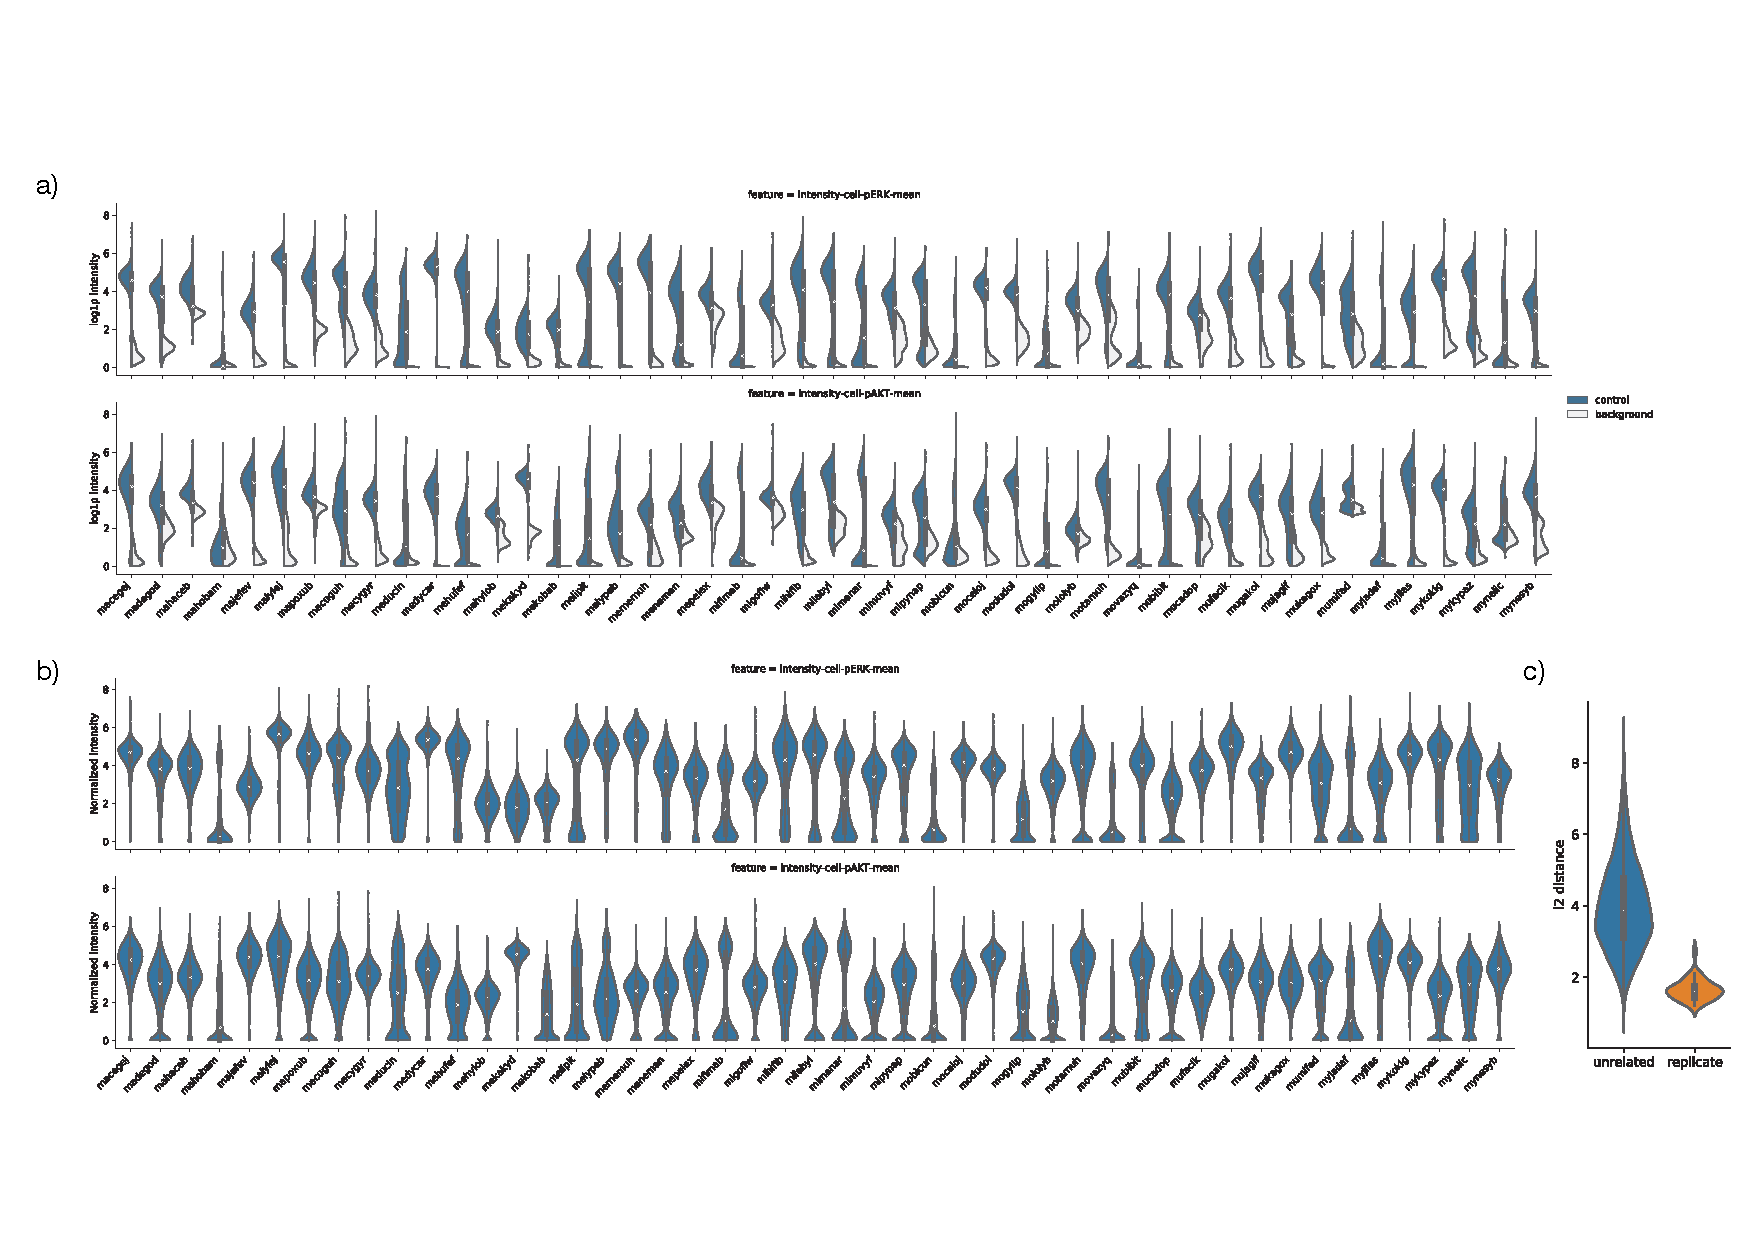
\includegraphics[width=0.95\textwidth]{figures/cellot-cohort/supplement/normalization.pdf}
  \end{center}
  \caption{
  Cohort normalization by removal of background intensity.
  a) distribution of intensity values of two features (pERK, top and pAKT, bottom) in the control state and secondary control (background). The secondary control measures the intensity generated when the probe is missing, considered to be uninformative "background" noise.
  b) Distribution of control intensities after removal of background intensity.
  c) For each patient the average state for all treatments are taken. Then within each condition, patient-patient similarities are computed as the euclidean distance between their averages. Replicates are much closer than unrelated samples, suggesting that the normalization has worked.
  }
\label{fig:cellot-cohort-normalization}
\end{figure}

\begin{figure}[h]
  \begin{center}
    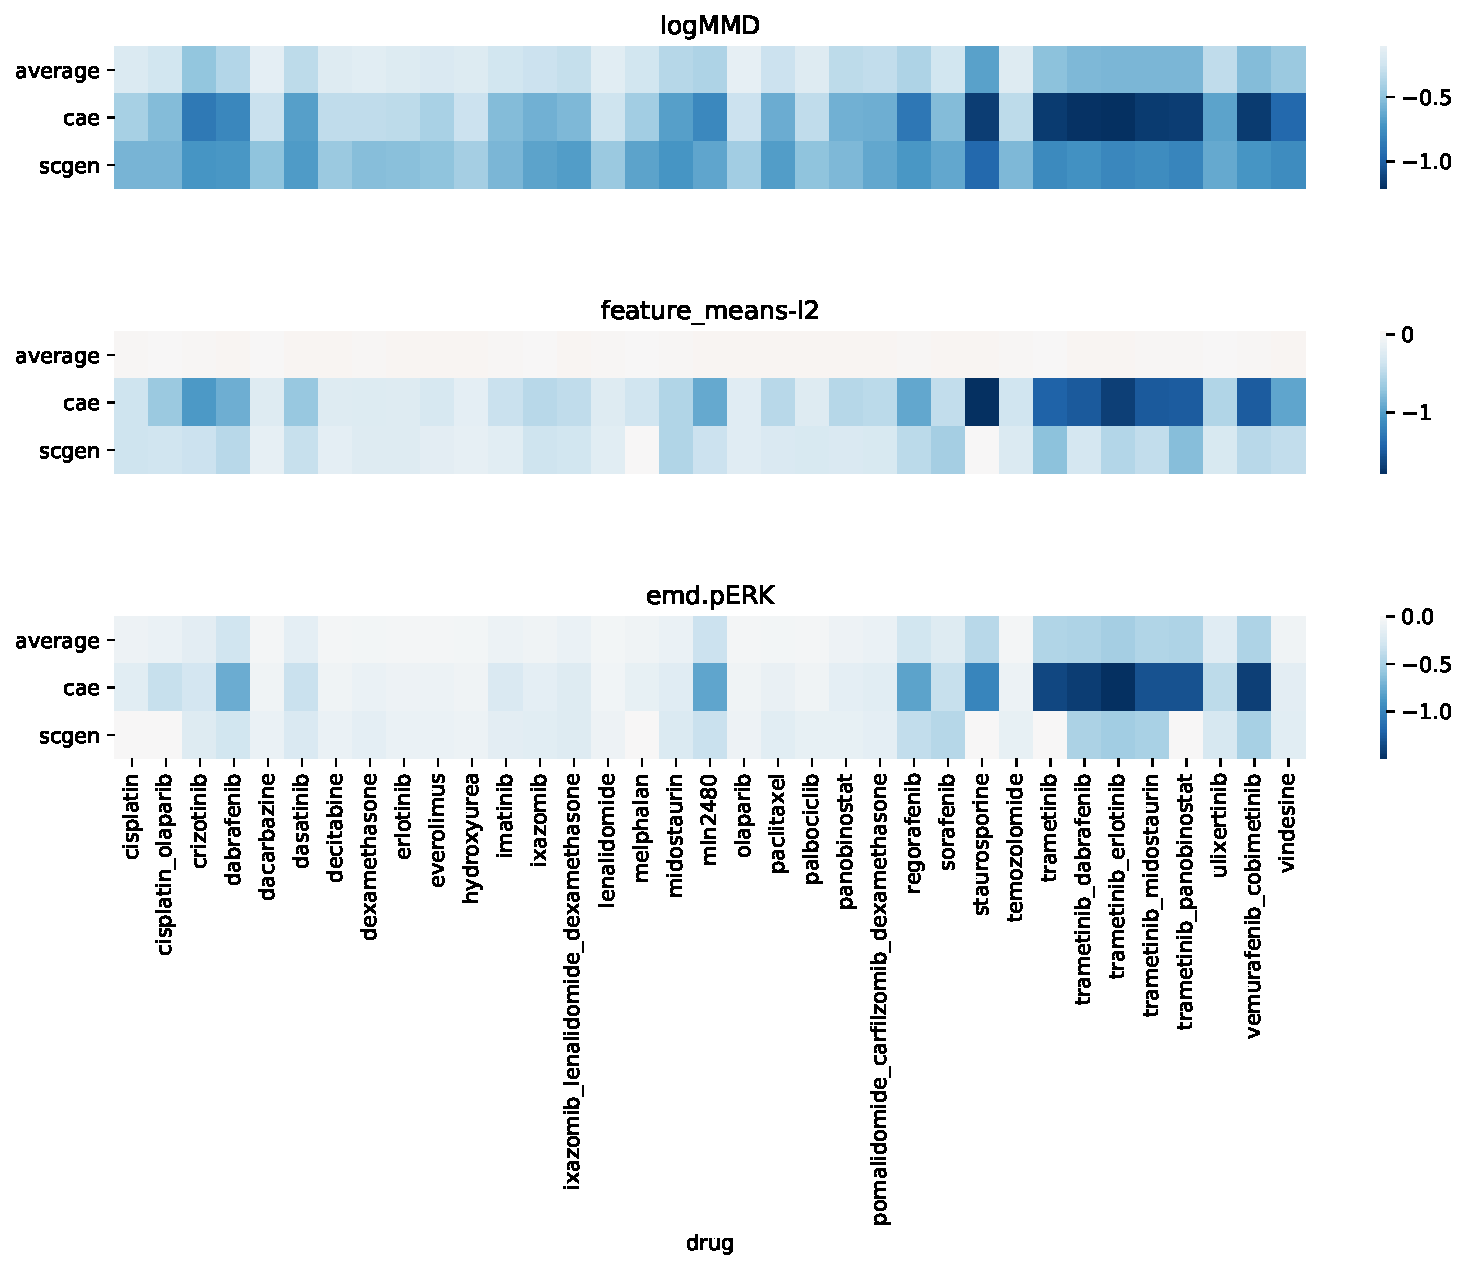
\includegraphics[width=0.95\textwidth]{figures/cellot-cohort/supplement/iid-metrics-drugs}
  \end{center}
  \caption{\textsc{CellOT} consistently improves metrics computed to compare (iid) predicted cell states with observed treated cell states.
  Three metrics are considered (MMD, euclidean distance between feature means and the EMD of pERK). 
  Colored squares indicate that there is a significant difference (t-test, $p < 0.01$ between \textsc{CellOT} and the baseline over the whole cohort.
  Blue hues indicate that \textsc{CellOT} improves over the baseline.
  }\label{fig:cellot-cohort-iid-metrics}
\end{figure}

\begin{figure}[h]
  \begin{center}
    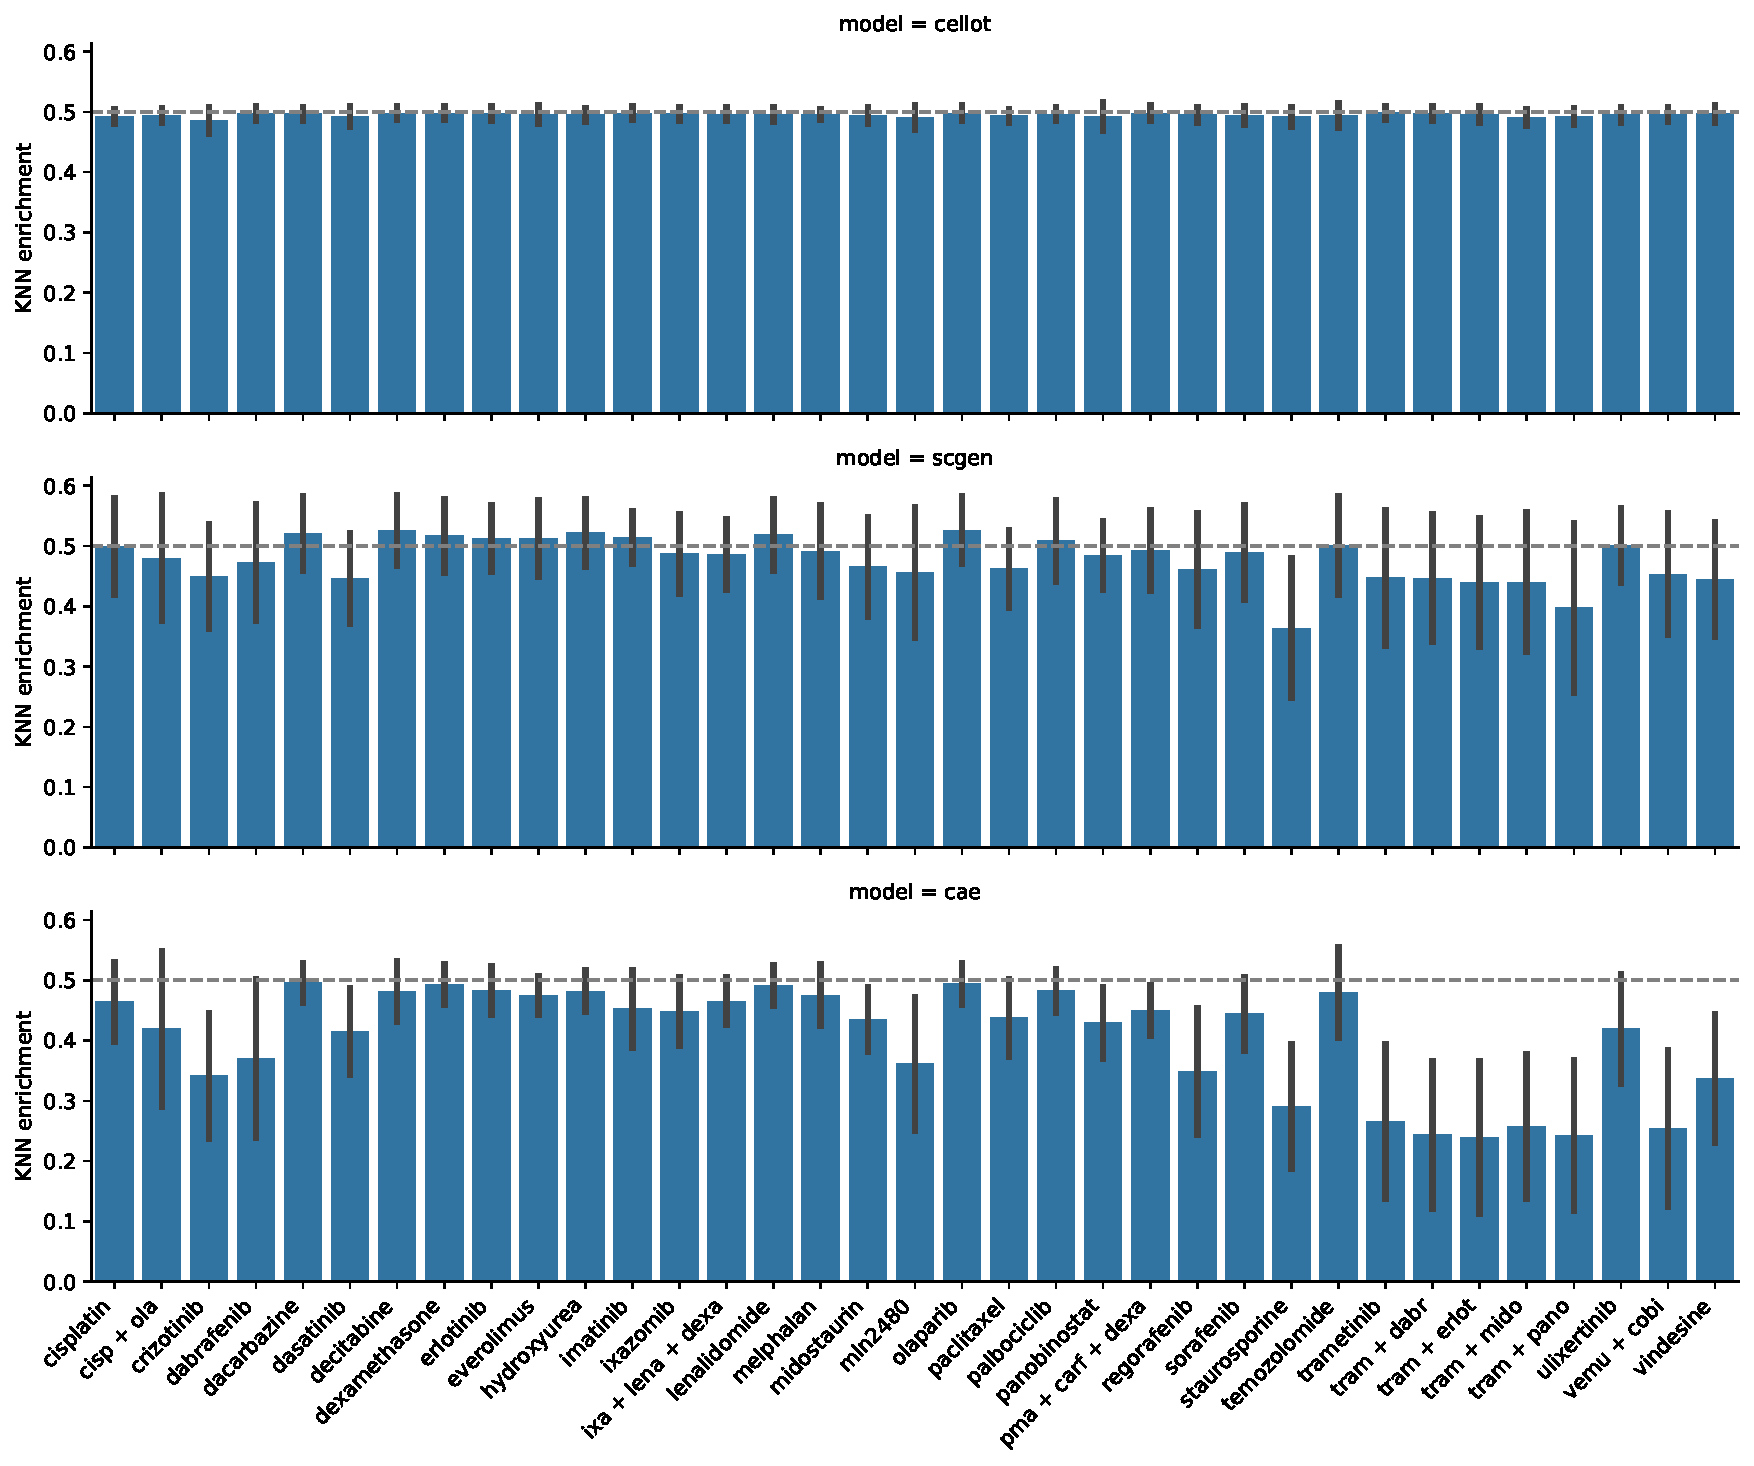
\includegraphics[width=0.95\textwidth]{figures/cellot-cohort/supplement/knn-enrichment-iid.pdf}
  \end{center}
  \caption{
  kNN enrichment scores (k=50) of predicted cells given an even mixtures of predicted and treated cells. For each sample, nearest neighbors are computed over an even split of treated and (i.i.d.) predicted cells for each treatment. Barplots are drawn over the distribution of average enrichment score for each treatment. Scores $< 0.5$ indicate that predicted states are grouped more with each other in isolation and thus do not faithfully represent the observed treated states.
  }
\label{fig:cellot-cohort-iid-knn}
\end{figure}

\begin{figure}[h]
  \begin{center}
    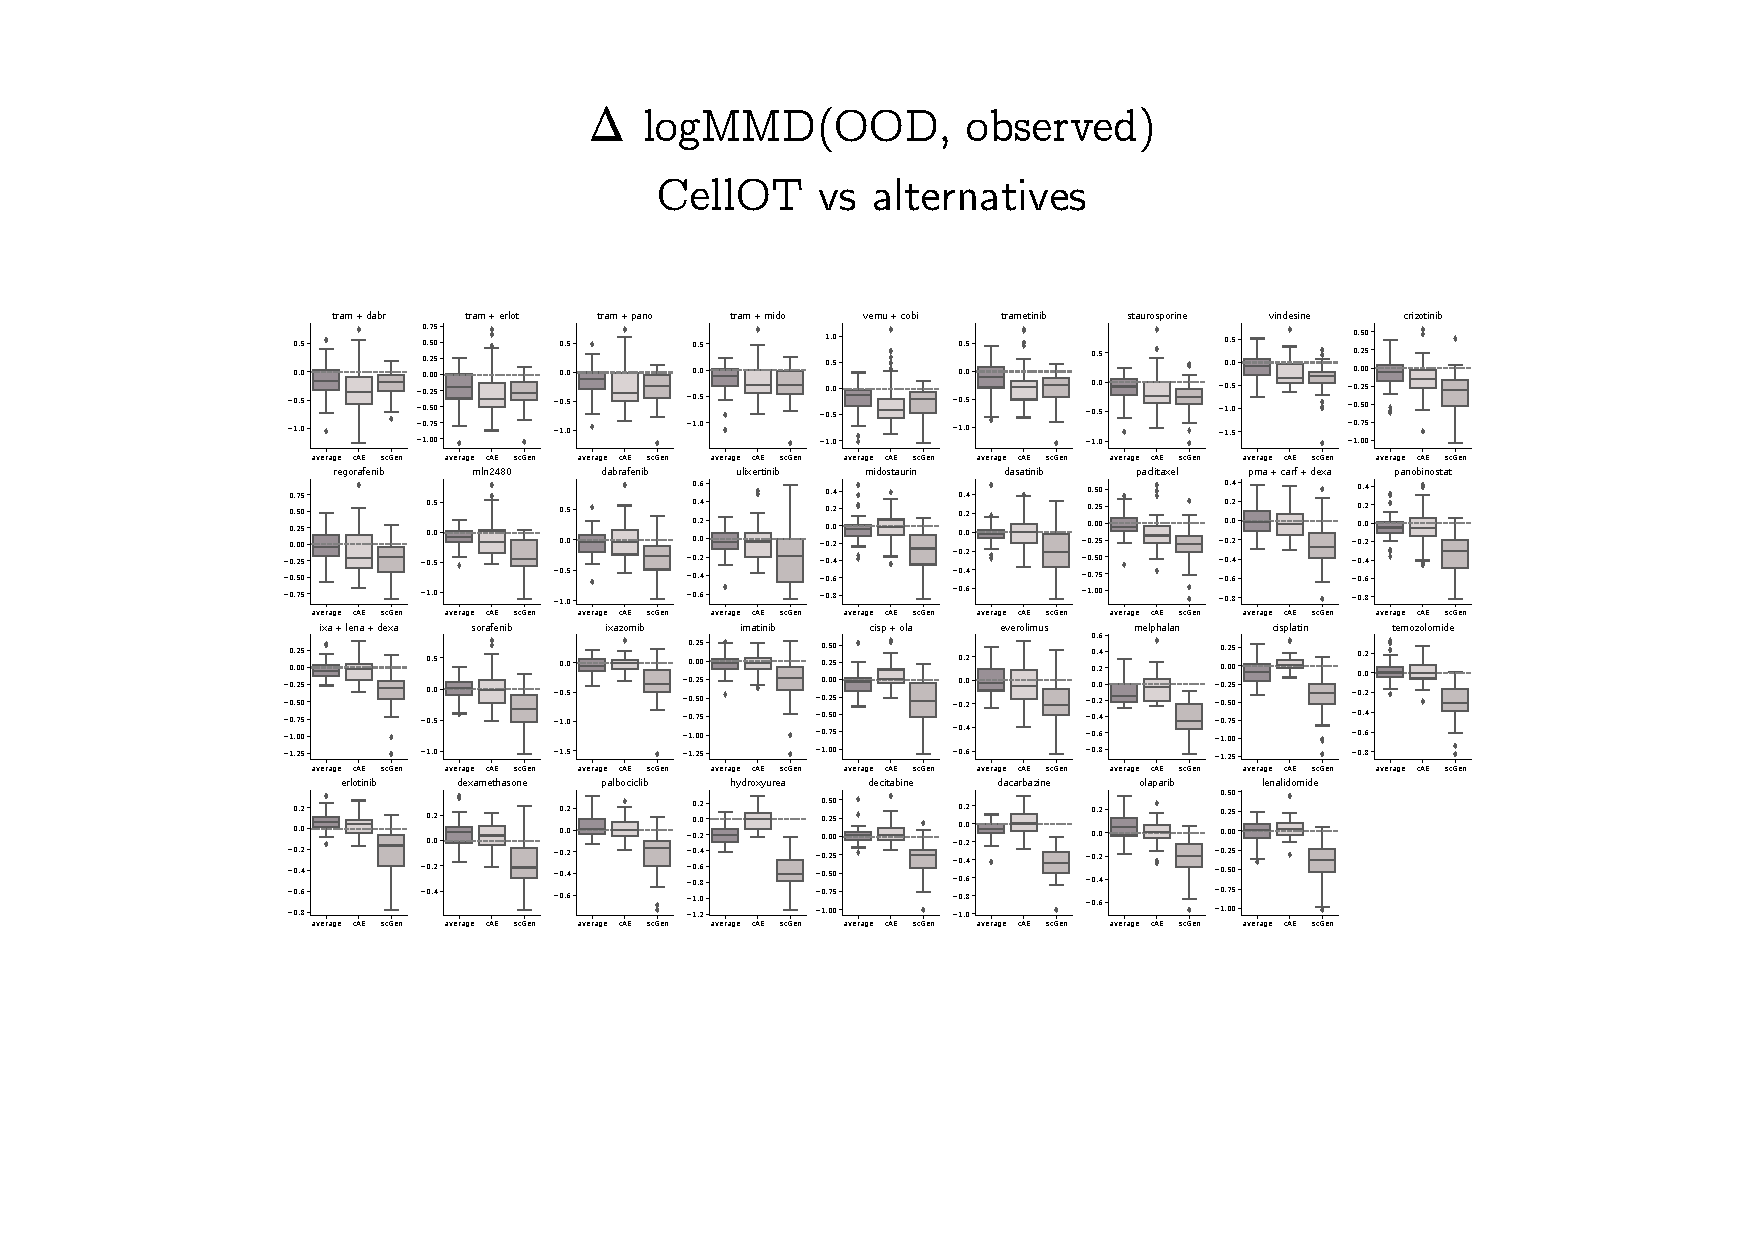
\includegraphics[width=0.95\textwidth]{figures/cellot-cohort/ood-eval-logmmd.pdf}
  \end{center}
  \caption{
    Pairwise logMMD differences comparing \textsc{CellOT} and baseline approaches.
    For each (drug, patient) pair, models are trained on the entire cohort with that patient held out.
    Each model predicts the drug response of the heldout patient
    and logMMD values are computed between the distribution of predicted treated states and the true treated states.
    Negative values correspond to settings where \textsc{CellOT} improves over the corresponding baseline.
  }
\label{fig:ood-eval-logmmd}
\end{figure}

\begin{figure}[h]
  \begin{center}
    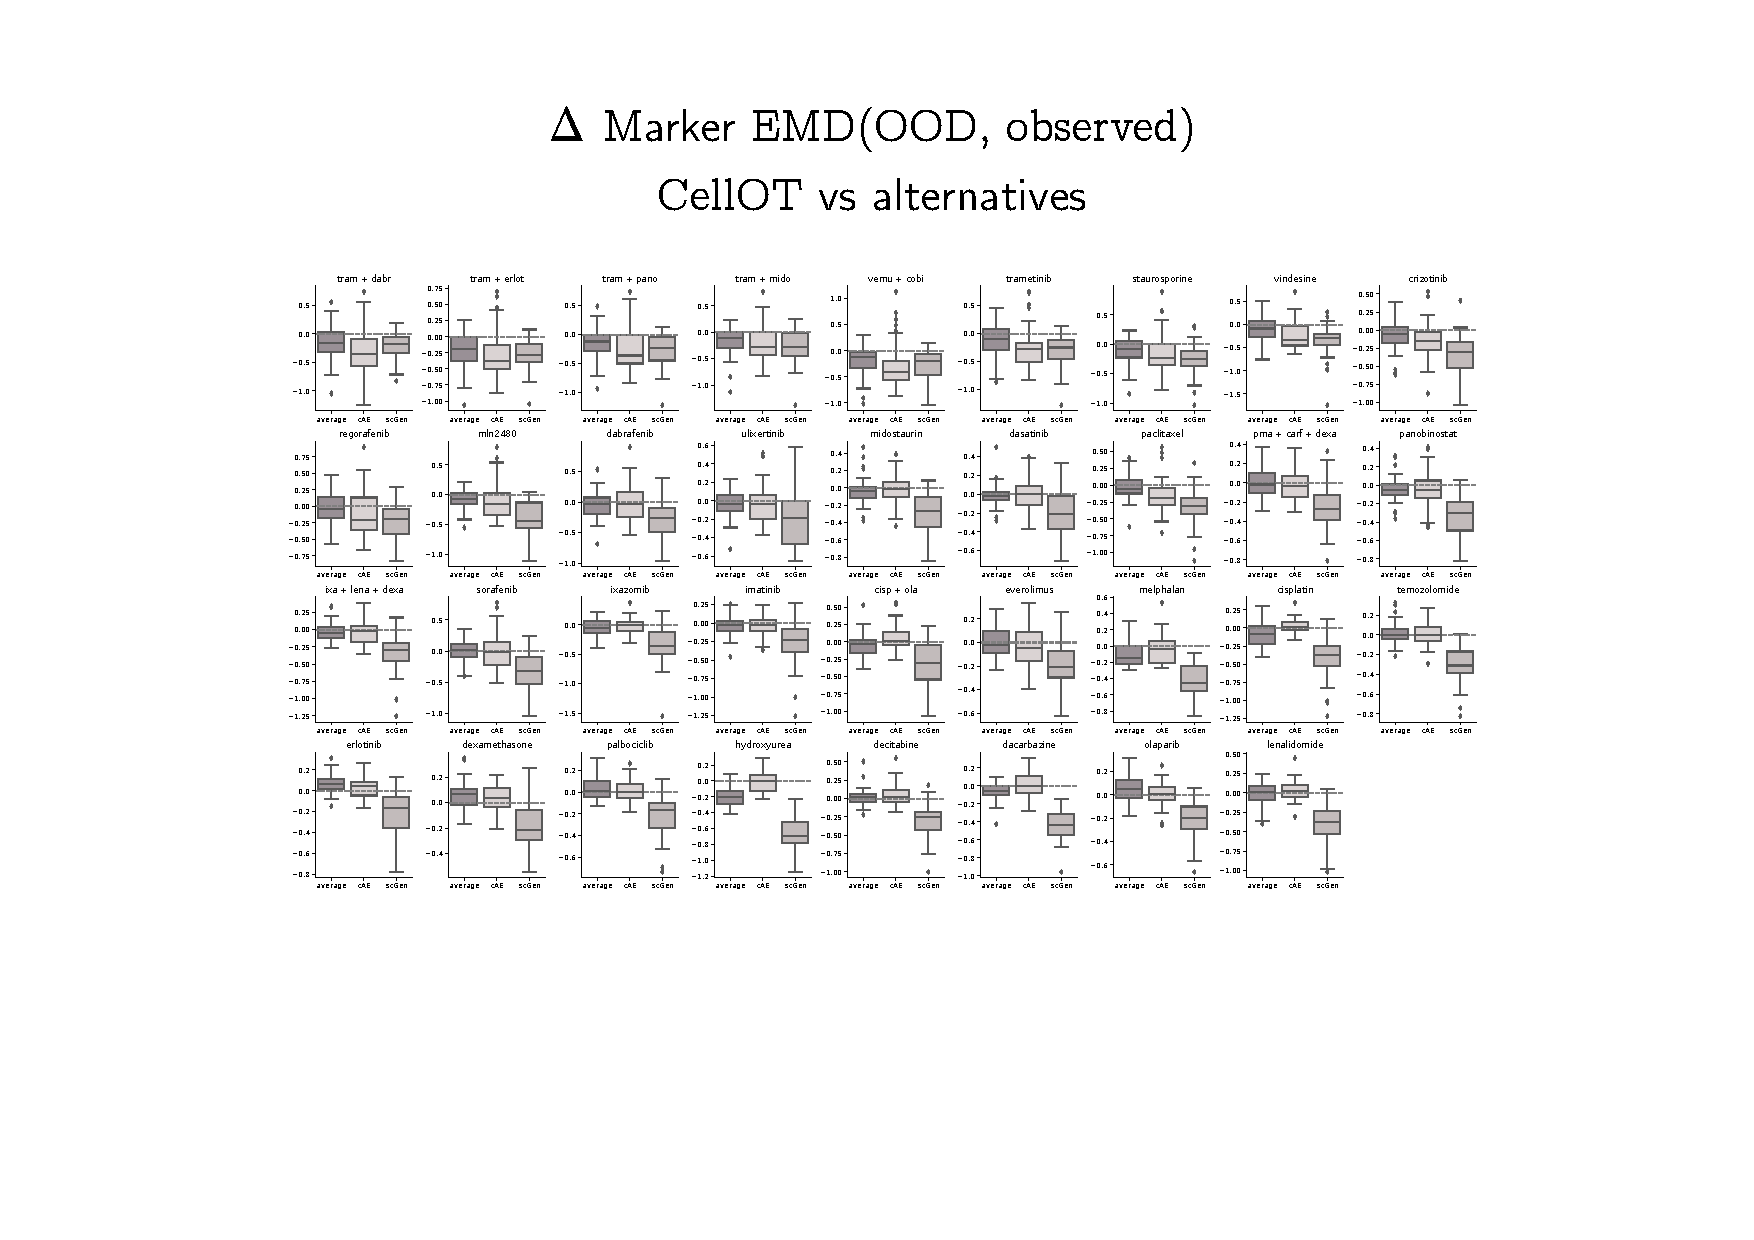
\includegraphics[width=0.95\textwidth]{figures/cellot-cohort/ood-eval-marker.pdf}
  \end{center}
  \caption{
    Pairwise marker EMD differences comparing $\textsc{CellOT}$ and baseline approaches.
    For each (drug, patient) pair, models are trained on the entire cohort with that patient held out.
    Each model predicts the drug response of the heldout patient
    and marker EMD values are computed between the distribution of predicted treated states and the true treated states.
    Negative values correspond to settings where $\textsc{CellOT}$ improves over the corresponding baseline.
  }
  \label{fig:ood-eval-marker}
\end{figure}

\begin{figure}
  \begin{center}
    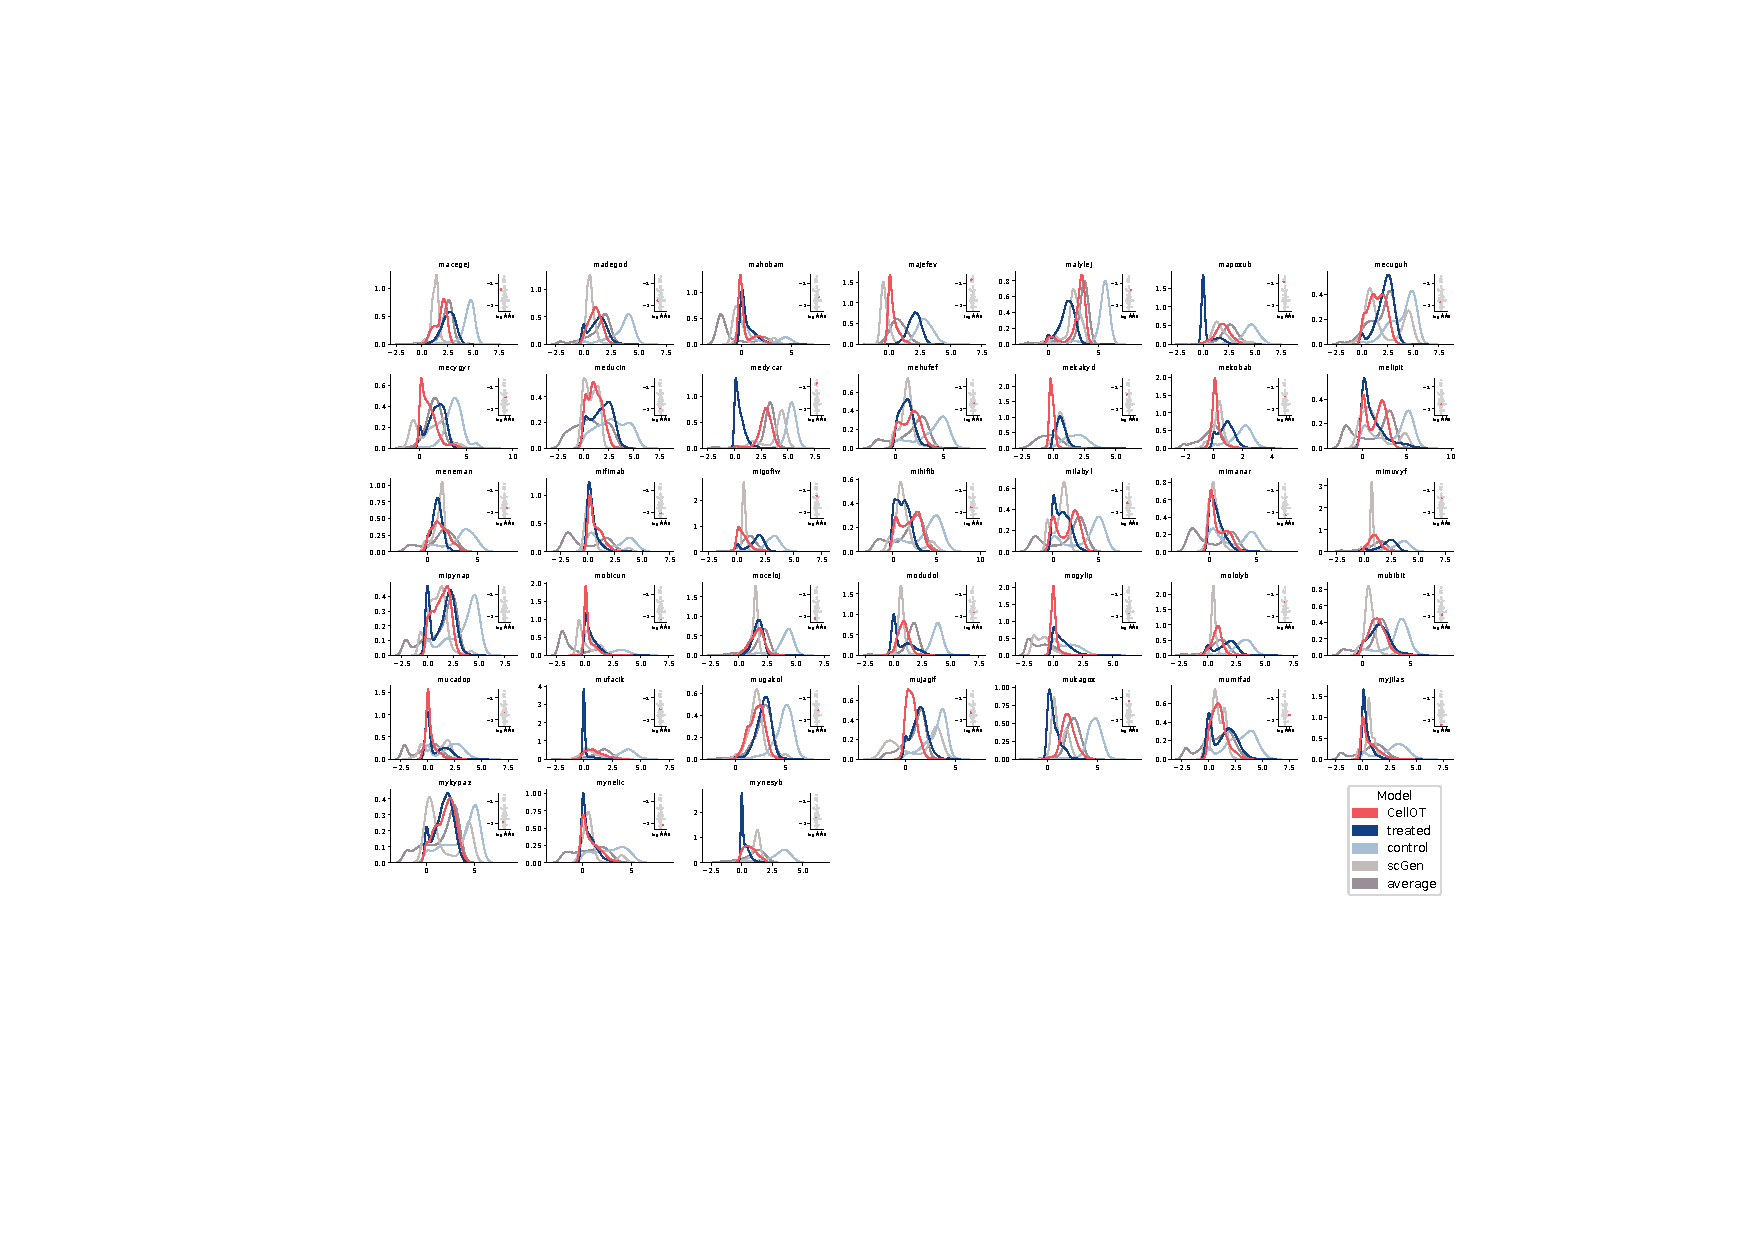
\includegraphics[width=0.95\textwidth]{figures/cellot-cohort/ood-predict-marginals.pdf}
  \end{center}
  \caption{
    Predicted response to trametinib dabrafenib combination treatment of each heldout samples.
    Marginals are shown for the treatment's marker feature, pERK.
    The inlay shows the selected heldout sample's logMMD score against the rest of the cohort.
  }\label{fig:ood-predict-marginals}
\end{figure}

\begin{figure}
  \begin{center}
    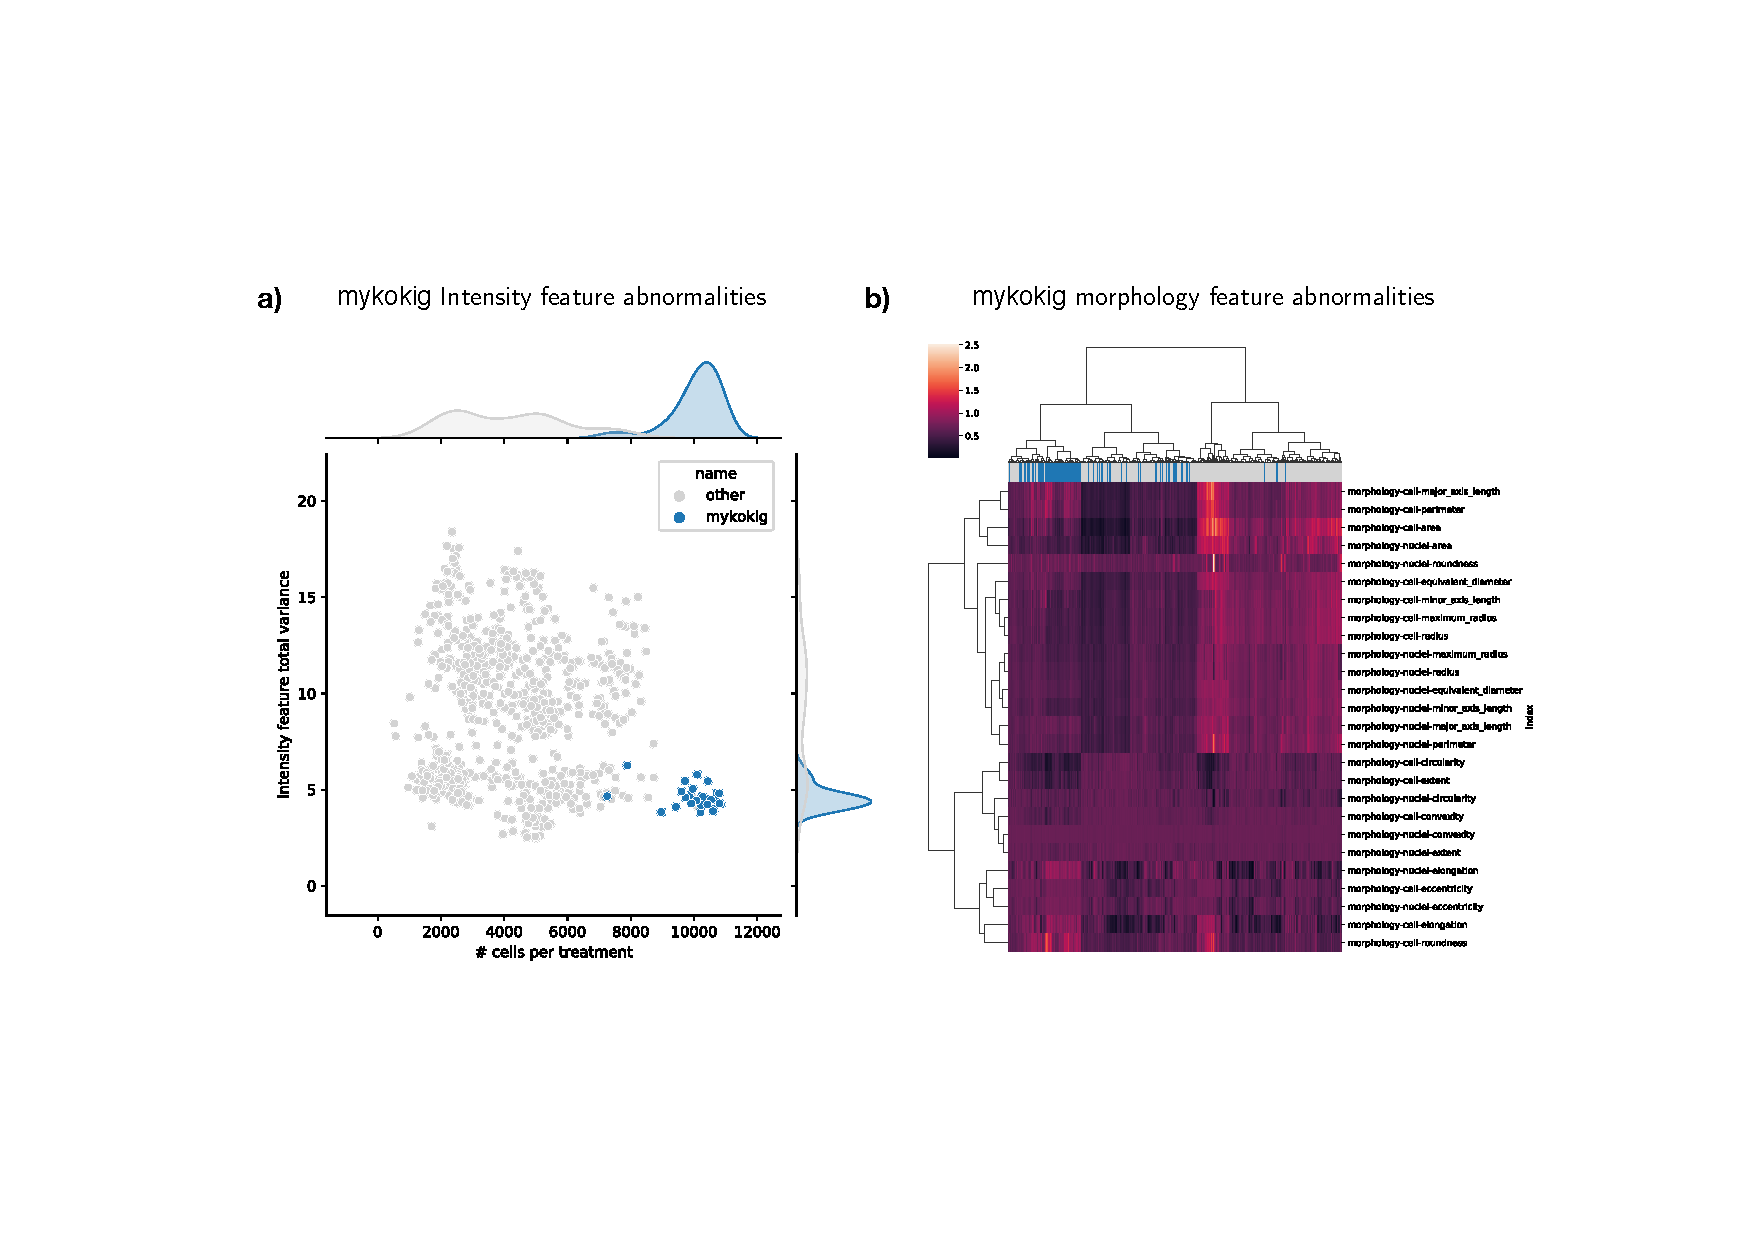
\includegraphics[width=0.95\textwidth]{figures/cellot-cohort/progression-exclude-mykokig.pdf}
  \end{center}
  \caption{
    Sample mykokig exhibits evidence for low quality cell segmentation and is removed from the progression prediction task.
  a) Scatter plot of number of treated cells by the variance of intensity features.  Each dot corresponds to a (treatment, sample) pair and treatments of mykokig are shown in blue. Mykokig behaves as an outlier as it has much more cells per treatment than other samples and these cells have low variance in their intensity features.
  b) Morphology features of mykokig cells indicate the presence of artifacts. The cluster map shows the distribution of each extracted morphology feature (rows) for cells sampled from mykokig and a subset of 5 samples from the full cohort. A large fraction of mykokig cells exhibit a strange unique morphology pattern of small round cells.
  }\label{fig:progression-exclude-mykokig}
\end{figure}

\begin{figure}
  \begin{center}
    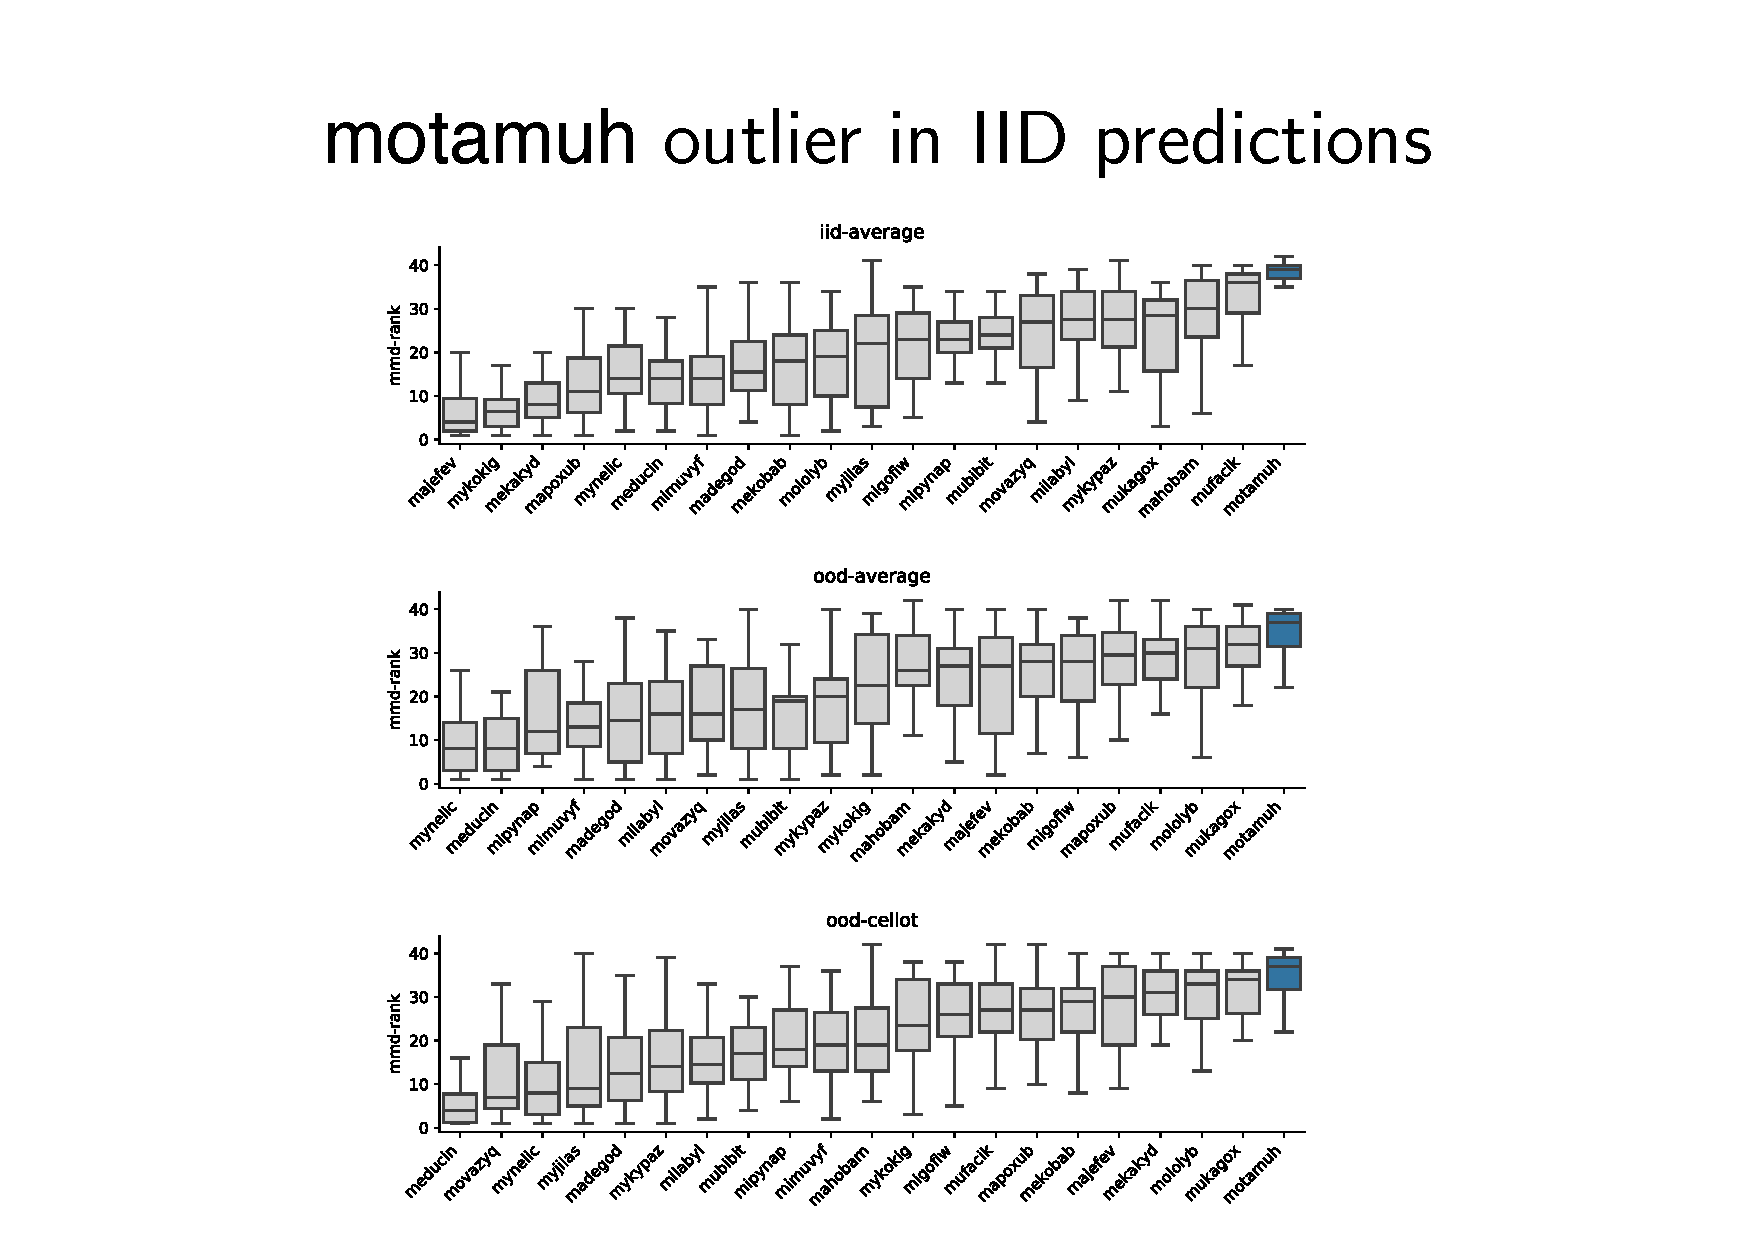
\includegraphics[width=0.95\textwidth]{figures/cellot-cohort/progression-exclude-motamuh.pdf}
  \end{center}
  \caption{
    The predicted responses for sample motamuh are consistently poor and the sample is therefore removed from the progression prediction task.
    Boxplots show the ranked MMD metric computed between each model's prediction and observed treated states for drugs considered in the progression prediction task.
    Results for the average model are shown in the IID and OOD setting as well as CellOT predictions in the OOD setting.
    Sample motamuh consistently ranks worst across all samples in the cohort for these prediction tasks.
  }\label{fig:progression-exclude-motamuh}
\end{figure}

\begin{figure}[h]
  \begin{center}
    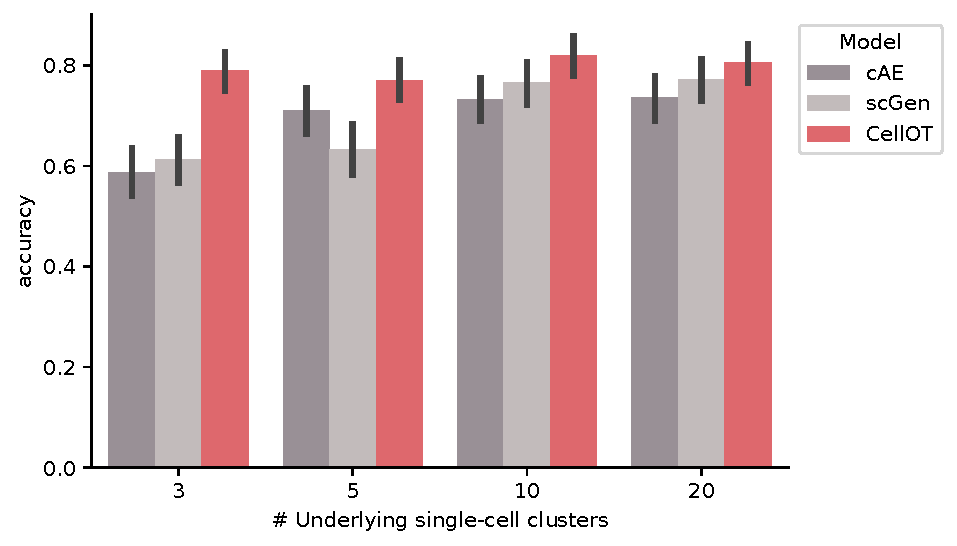
\includegraphics[width=0.95\textwidth]{figures/cellot-cohort/supplement/survival-accuracies-baselines.pdf}
  \end{center}
  \caption{Progression prediction, ablation of model against number of underlying clusters and prediction model used. Baseline models do not improve over \textsc{CellOT}, which is also much less sensitive to the choice of hyperparameter, indicating that \textsc{CellOT} scDRs have a high information content.
  }
\label{fig:survival-accuracies}
\end{figure}
